
\subsection{Skyline Query}\label{sec:skyline_operator}

Skyline query is an operation that finds all data records that
are not dominated by any other data records in a given data set. A
record dominates another record if it is as good or better in all
dimensions and better in at least one dimension. Skyline query is
closely related to the maximal vector
problem~\cite{journals/jacm/KungLP75,conf/vldb/GodfreySG05}. Here,
we briefly introduce these concepts.

\begin{definition}[Maximal Vector]\label{def:max_vector}
Given the set of vectors $V$, for $v \in V$, if there does not
exist $u \in V$ such that $u$ $\geq$ $v$ and $u$ $\neq$ $v$, then
$v$ is a maximal vector of $V$.

\begin{equation}\label{eq:max_vector}
    MaxVect(V) = \{v | \forall v, u \in V \mbox{ } \nexists u \geq v\}
\end{equation}

\end{definition}

The comparison operator $\geq$ utilized in
Equation~\ref{eq:max_vector} is defined on vectors such that for
two vectors $u$, $v \in V$, $u$ $\geq$ $v$ if $u_i$ $\geq$ $v_i$
for $i$ = 1 to $n$ and vice versa for the $\leq$ operator. In
other words, a vector $v$ is greater than the other vector $u$ if
and only if all elements of $v$ is \emph{greater than or equal to}
all elements of $u$. The comparison operators for each element of
the vectors are the natural ordering operators defined on each
domain.

The main difference between the maximal vector operation defined
in Definition~\ref{def:max_vector} and the skyline operation is
that the skyline operator defines a set of \emph{preference
specifiers}, $\sigma$, which are to be either \emph{minimal}
(\emph{min}) or \emph{maximal} (\emph{max}) for each dimension.


\begin{definition}[Skyline Operator]\label{def:skyline}
Give a set of tuples, $T$, and a set of preference specifiers,
$\sigma$, the skyline operator is defined as follows:

\begin{equation}\label{eq:skyline}
    Skyline(T, \sigma) = \{t \in T | \nexists s \in T \text{ where } s \succ t \}
\end{equation}

\end{definition}

The dominance relationship $\succ$ in Definition~\ref{def:skyline}
is defined in the following definition.

\begin{definition}[Dominance Relationship]\label{def:dom_rel}
Given two tuples $t_1$ and $t_2$ in $T$, $t_1$ dominates $t_2$ if
and only if all attributes of $t_1$ dominate or equal all
attributes of $t_2$ and at least one attribute of $t_1$ dominates.
Dominance for each attribute depends on the preference specifier,
$\sigma_i$, for that attribute. Given $x$ and $y$ from a certain
domain $D_i$, the dominance for the attributes is defined as
follows:

\begin{enumerate}
\item If $\sigma_i$ = \emph{min}, $x$ dominates $y$ if $x$ $<$
$y$. \item If $\sigma_i$ = \emph{max}, $x$ dominates $y$ if $x$
$>$ $y$.
\end{enumerate}
\end{definition}



%\begin{corollary}\label{co:dom_rel}
%The dominance relationship is transitive, non-reflexive, and
%non-symmetric.
%\end{corollary}

%\begin{proof}
%All three properties can be proven based on the fact that the
%values of each attribute domain are ordered: an attribute $x$ is
%better than $y$ then, $y$ is worse than $x$. The transitive
%property of the dominance relationship follows from
%Definition~\ref{def:dom_rel}, if record $A$ dominates $B$ then all
%attributes of $A$ are equal or better and there is at least one
%attribute that is better; therefore, $B$ dominates $C$ implies
%that all attributes of $A$ is equal or better than $C$ therefore,
%the relationship is transitive. The relationship is non-reflexive
%since if all attribute of $A$ is equal or better than attribute of
%$B$ then the ordering of the values of each attribute domain imply
%that $B$ does not dominate $A$. Similarly, $D$ does not dominate
%itself since the definition states that at least one must be
%better for a record to dominate another.
%\end{proof}
%
%Following the non-reflexive property of
%Corollary~\ref{co:dom_rel}, given two record $A$ and $B$ and $A =
%B$, if $A$ is a skyline record, then $B$ is also a skyline record.
%
%Skyline constraint regions was introduced in
%\cite{conf/dexa/HaKCL09}. Constraint region limits the skyline
%queries to a subset of the data set instead of the entire data
%set. For example, a constraint could be a limit of hotel price
%within the range \$100 to \$150 and the distance within 0 to 3
%miles from the beach. Constraint region is a separate issue in
%skyline queries that can be easily satisfied with a filtering step
%to remove all tuples not in the region preceding the main skyline
%algorithm. In this chapter, we do not consider constraint region,
%and assume the entire space of the data set as the search space.


\subsection{Wireless Data Broadcast}\label{sec:wireless_broadcast}

A wireless data broadcast environment consists of a broadcast
channel, a broadcast server, and mobile clients who are interested
in the broadcast program from the server. The server is the
originator of the broadcast program which contains relevant data
records and pushes the data onto the channel. The mobile clients
receive desired data by listening to the channel. Examples of
services such as XM Satellite
Radio\footnote{http://www.siriusxm.com/} and Microsoft MSN Direct.
The model is illustrated in Figure~\ref{fig:broadcast}.

\begin{figure}[!h]
\begin{center}
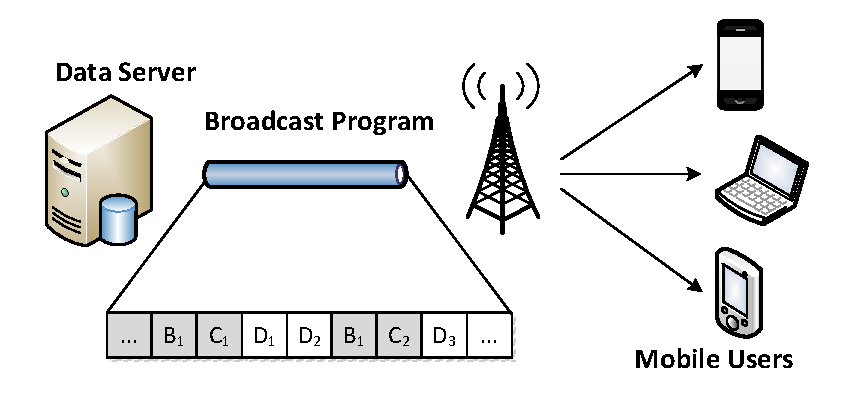
\includegraphics[width=3.5in]{Figures/on_demand.eps}
\vspace*{-5pt} \caption{A wireless broadcast environment.}
\vspace*{-10pt} \label{fig:broadcast}
\end{center}
\end{figure}

A complete dissemination of all the records in the data set from
the server is a \emph{broadcast cycle}. A cycle follows another
cycle (see Figure~\ref{fig:bcastcycle}). In this chapter, we use the
terms cycle and program interchangeably to denote the content of
the broadcast channel.

An inherent challenge of the broadcast model is the forward only
data model; there is no random access of the data set. When a
client misses a piece of data from the current cycle, the client
must wait until the next cycle. The influences of these properties
on the broadcast environment are: (1) we cannot adopt skyline
algorithms designed for disk-based database systems that require
random data access, and (2) we must design a self-explanatory
broadcast program using indexes.

Many previous studies have been done on different broadcast
environments. Multi-channel broadcast for data dissemination (and
techniques of data allocation) has been studied
in~\cite{conf/cikm/HsuLC01,conf/cikm/YeeN03,conf/mobicom/HameedV97}.
Adaptive broadcast systems that allow limited uplink (client to
server) communication have been surveyed
in~\cite{journals/pieee/Wong88}. In this chapter, we assume the
following properties for our broadcast environment: (1) a channel
is forward-only, (2) only one channel is utilized, and (3) no
uplink from clients to server.

\begin{figure}[!h]
\begin{center}
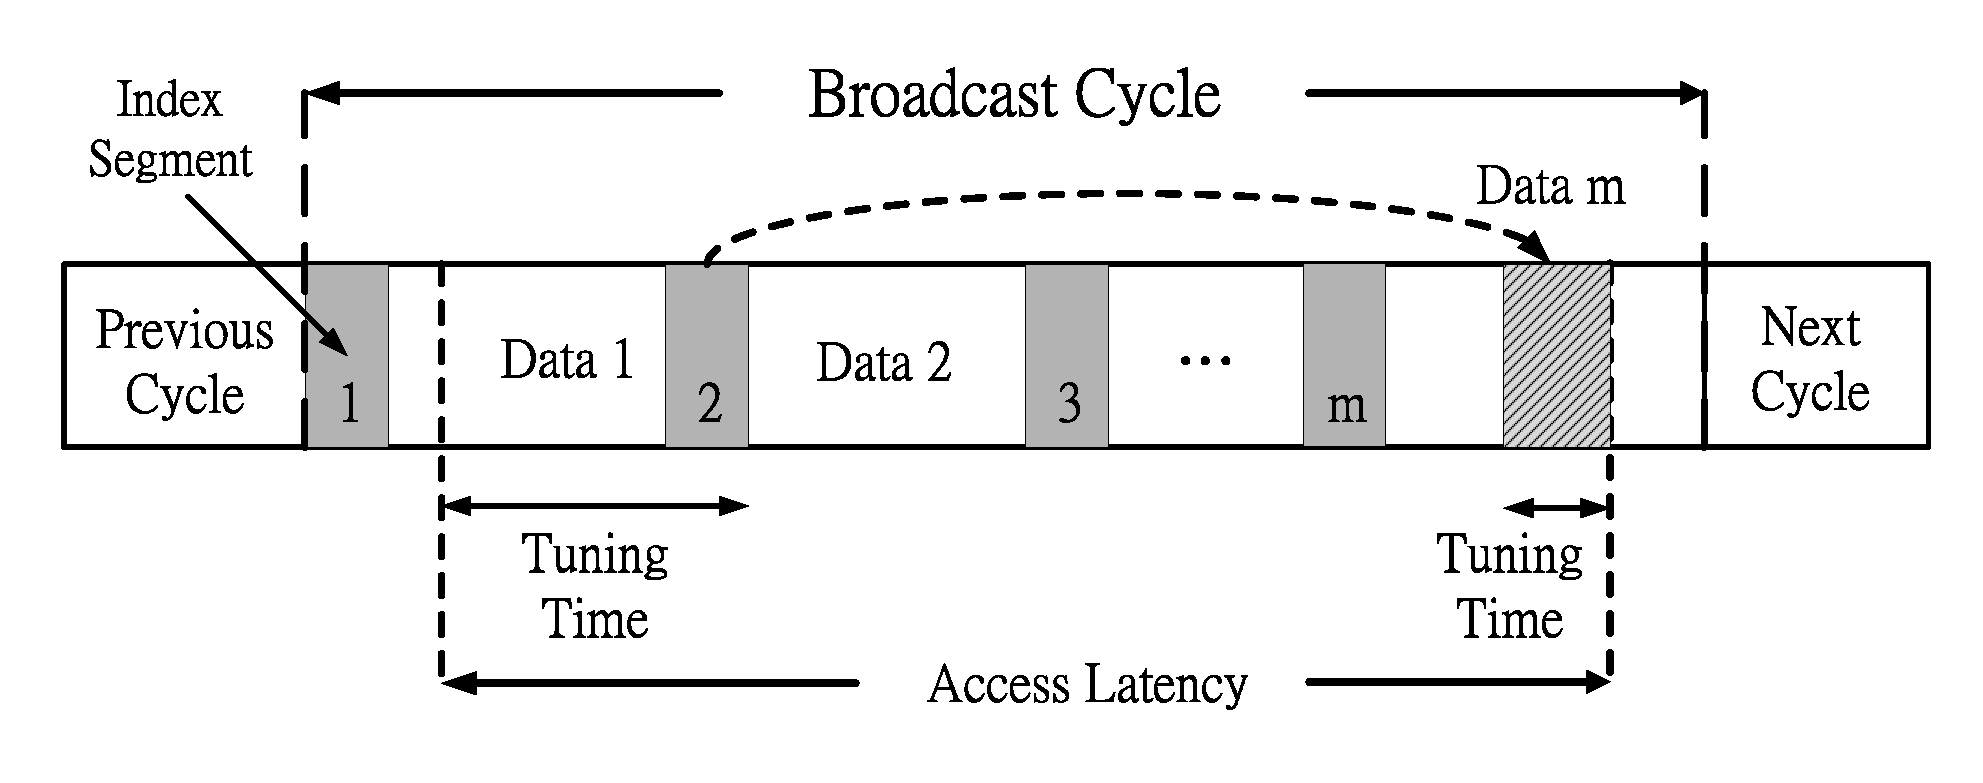
\includegraphics[width=4in]{Figures/BroadcastCycle.eps}
\vspace*{-15pt} \caption{Broadcast program cycles.}\vspace*{-10pt}
\label{fig:bcastcycle}
\end{center}
\end{figure}

Power consumption is a major concern in wireless broadcast
environments since most clients are mobile devices, such as
cellular phones, powered by a small battery. Therefore, power is a
scarce and valuable resource for these devices; continuously
listening to the broadcast channel is expensive in terms of power
usage. Most mobile devices are able to turn off the radio receiver
when they are not actively receiving data to conserve power. To
reduce power consumption, an index is used to make the broadcast
cycle self-descriptive. As depicted in
Figure~\ref{fig:index_node}, an index provides additional
information in a broadcast program to tell the clients the
approximate time that a data record will be broadcast. A broadcast
index is analogous to an index in traditional databases in which
the indexes provide the location of data records and facilitate
fast lookup of records. With the index information, the clients
can turn off the radio receiver to conserve power and only tune
into the channel when the desired data is being broadcast.

\begin{figure}[!h]
\centering \subfigure[Data set.]{
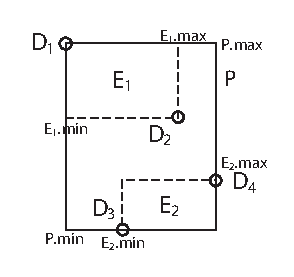
\includegraphics[width=2in]{Figures/mbr_2d.eps}
\label{fig:mbr_2d} } \subfigure[On air index.]{
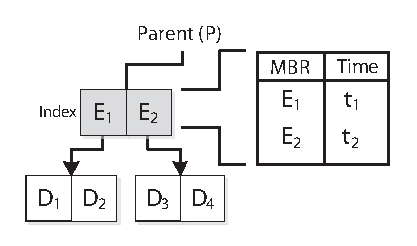
\includegraphics[width=2in]{Figures/index_node_entry.eps}
}\vspace*{-10pt} \caption{A sample broadcast index.}
\label{fig:index_node}
\end{figure}

Adding an index to a broadcast cycle also adds space overhead to
the cycle and consumes broadcast bandwidth. Quantities that
measure the efficiency of a wireless broadcast program are defined
below. \emph{Access latency} and \emph{tuning time} are well-known
metrics of the broadcast model and have been studied
in~\cite{journals/vldb/ZhengLLLS09,journals/tkde/ImielinskiVB97,
conf/icde/KuZW07,journals/tmc/KuZW08,journals/winet/LeeL99}. We
also define \emph{index percentage} and \emph{initial index probe}
as measurements of index space overhead and index probe latency.

\begin{definition}[Access latency]\label{def:access_latency}
The amount of time from when a client requests data to the point
when the client receives all the desired data. This quantity is
denoted by $\alpha$.
\end{definition}

\begin{definition}[Tuning time]\label{def:tuning_time}
The total amount of time a client actively listens to the channel.
The time determines the power consumed by the client to retrieve
the required data. The quantity is denoted by $\tau$.
\end{definition}

Both the access latency and the tuning time are measured in terms
of number of data packets.

\begin{definition}[Index percentage]\label{def:index_percentage}
The ratio of the space allocated to the index to the space of the
entire cycle measures in bytes. This quantity is defined as $\rho
= \frac{\delta}{\omega}$.
\end{definition}

\begin{definition}[Initial index probe]\label{def:index_probe}
The amount of time for a client to get to the first index segment.
This quantity is denoted by $\lambda$.
\end{definition}


\begin{table}[!h]
\centering \caption{Summary of notations.} \vspace*{5pt}
\label{tab:index_attr}
\begin{tabular}{|c|p{2.45in}|}
\hline
{\bf Notation} & {\bf Description}\\
\hline\hline
$n$ & Number of dimensions of skyline \\
$m$ & Number of index segments in a cycle \\
$D$ & A set of attribute domains $D$ = \{$d_1$, ..., $d_n$\} \\
$T$ & A set of records (tuples) \\
%$p$ & A record (a n-tuple) \\
%$S$ & A set of skyline points \\
$\sigma$ & A set of skyline preference specifiers \\
%$R$ & A pruning region \\
$B$ & A minimal bounding box (MBR) \\
$E$ & An R-tree index entry (MBR, time) \\
$b$ & Branching factor of an index tree \\
$h$ & Height of an index tree \\
%$L$ & Tree level \\
$L_r$ & Levels of index tree replication \\
$\rho$ & Index percentage \\
%$\alpha$ & Initial index probe \\
$\alpha$ & Access latency \\
$\tau$ & Tuning time \\
$\delta$ & Size of a broadcast index \\
$\theta$ & Size of a broadcast data set \\
$\omega$ & Size of an entire program cycle $\delta + \theta$ \\
\hline
\end{tabular}
\end{table}

\begin{comment}
\begin{mydef}[Constraint Skyline] Give a set of spatial constraints
    $C$ = \{$c_1$, $c_2$, ..., $c_n$\}
    \begin{equation}
    ConsSkyline(P) = Skyline(P), \\where p \epsilon P~satisfies~C
    \end{equation}
\end{mydef}
\end{comment}
